\documentclass{article}
\usepackage{amsmath, amssymb, amsthm, enumitem}
\usepackage{fullpage}
\usepackage{tikz}
\newtheorem{corollary}{Corollary}
\usepackage{amsthm}
\newtheorem{lemma}{Lemma}
\usepackage{microtype}
\usepackage{polynom}
\usepackage{placeins}
\usepackage{tikz}
\usepackage{forest}
\usetikzlibrary{trees}


\title{Discrete Mathematics 1 Lectures, Part 1}
\author{Tomasz Brengos \\  
Committers : Aliaksei Kudzelka, Mykhailo Moroz, Mihail Orlov}
\date{}

\begin{document}
\maketitle

\section{Counting (Combinatorics)}

Counting forms the basis of combinatorics. In these lectures we explore several counting rules, examples, and proofs.

\subsection{Rule of Sum (Addition Principle)}
If a set $S$ is partitioned into disjoint subsets,
\[
S = S_1 \cup S_2 \cup \cdots \cup S_k,
\]
then the total number of elements in $S$ is the sum of the number of elements in each subset:
\[
|S| = |S_1| + |S_2| + \cdots + |S_k|.
\]

\paragraph{Example:}  
Suppose we wish to count the number of ways to choose a subset of a set $X$ of size $u$, but we only consider subsets of a fixed size $k$. If we let $S$ be the family of all such subsets, then using the rule of sum by dividing the choices according to a distinguished element (say, whether a chosen element is included or not) we can count the subsets by summing over the possibilities. (This idea is used later in proofs for binomial coefficients and the power set.)

\paragraph{Theorem:}
\[
\binom{n}{k} = \binom{n-1}{k-1} + \binom{n-1}{k}
\]

\paragraph{Proof:}
Consider \( S = \binom{X}{k} \), the set of all subsets of \( X \) of size \( k \).  
Take any element \( a \in X \). Define:  
 \( S_1 \) as the subsets in \( S \) that contain \( a \) and  
 \( S_2 \) as the subsets in \( S \) that do not contain \( a \).  

Since every subset of \( S \) either contains \( a \) or does not, we see that \( S_1 \) and \( S_2 \) are disjoint and their union forms \( S \), i.e.,  
\[
S_1 \cup S_2 = S.
\]

By the rule of sum, we get:  
\[
|S| = |S_1| + |S_2|.
\]

Now,  
each subset in \( S_1 \) must contain \( a \), so we choose the remaining \( k-1 \) elements from \( X \setminus \{a\} \), which has \( n-1 \) elements. Thus, \( |S_1| = \binom{n-1}{k-1} \).  
Each subset in \( S_2 \) does not contain \( a \), so we choose all \( k \) elements from \( X \setminus \{a\} \). Thus, \( |S_2| = \binom{n-1}{k} \).  

Therefore,  
\[
\binom{n}{k} = |S| = |S_1| + |S_2| = \binom{n-1}{k-1} + \binom{n-1}{k}.
\]

\paragraph{Example:}  
Let \( S = \{ \triangle, \square, \circ \} \) and \( k = 2 \), choosing \( a = \circ \).  
Fixing \( \circ \) as one of the elements in the subset of size \( k \), we get:  
  \[
  S_1 = \{\{\circ, \triangle\}, \{\circ, \square\}\}.
  \]
Taking all subsets of size \( k \) without \( \circ \):  
  \[
  S_2 = \{\{\triangle, \square\}\}.
  \]
We have \( |S_1| = 2 \) and \( |S_2| = 1 \), so \( |S_1| + |S_2| = 3 \).  

\noindent On the other hand,  
\begin{align*}
\binom{3}{2} &= \frac{3!}{2!(3-2)!} = 3.
\end{align*}
Thus, \( |S| = |S_1| + |S_2| = 3 \), verifying the identity.  


\paragraph{}

\subsection{Rule of Product (Multiplication Principle)}
When an object is constructed by a sequence of choices, where:
\begin{itemize}[nosep]
    \item The first choice can be made in $a$ ways,
    \item The second in $b$ ways,
    \item $\ldots$
\end{itemize}
the total number of objects is the product:
\[
a \times b \times \cdots.
\]

\paragraph{Example:}  
A word of length $n$ over the binary alphabet $\{0,1\}$ is formed by choosing one of $2$ possibilities for each position. Hence, there are
\[
2^n
\]
possible words.

\subsection{Rule of Bijection}
If there exists a bijection (a one-to-one and onto mapping) between two sets $S$ and $T$, then they have the same number of elements:
\[
|S| = |T|.
\]

\paragraph{Example:}  
Consider the power set of a set $X$, denoted by $\mathcal{P}(X)$. There is a natural bijection between $\mathcal{P}(X)$ and the set of binary sequences of length $|X|$: for each subset $A \subseteq X$, assign the sequence $(a_1,a_2,\dots,a_n)$ where 
\[
a_i = \begin{cases} 
1, & \text{if } x_i \in A, \\
0, & \text{if } x_i \notin A.
\end{cases}
\]
This shows that 
\[
|\mathcal{P}(X)| = 2^{|X|}.
\]

\subsection{Counting in Two Ways}  

\paragraph{Rule of Counting in Two Ways}  
When two formulae enumerate the same quantity, they must be equal.  

\paragraph{Example:}  
\[
\sum_{i=1}^{n} i = \frac{n(n+1)}{2}
\]

\paragraph{Proof:}  
Consider a lattice grid of size \( (n+1) \times (n+1) \), defined as:  
\[
X = \{(i, j) \mid i, j \in \{1, 2, \dots, n+1\} \}.
\]  
Clearly, \( |X| = (n+1)^2 \).  

Now, partition \( X \) into three subsets:  
- \( X_1 \), the points strictly below the secondary diagonal.  
- \( X_2 \), the points strictly above the secondary diagonal.  
- \( X_3 \), the points on the secondary diagonal itself.  

Since these three sets form a partition, we have:  
\[
|X| = |X_1| + |X_2| + |X_3|.
\]  
Observing their sizes:  
\[
|X_1| = |X_2| = 1 + 2 + \dots + n, \quad |X_3| = n+1.
\]  
Thus,  
\[
(n+1)^2 = 2(1 + 2 + \dots + n) + (n+1).
\]  
Rearranging, we get:  
\[
1 + 2 + \dots + n = \frac{(n+1)^2 - (n+1)}{2} = \frac{n(n+1)}{2}.
\]

Hence, we have proven the formula:  
\[
\sum_{i=1}^{n} i = \frac{n(n+1)}{2}.
\]


\subsection{Binomial Coefficients and Permutations}
Let $X$ be a set with $|X| = n$.

\paragraph{Subsets:}  
The number of ways to choose a $k$-subset of $X$ is given by the binomial coefficient
\[
\binom{n}{k}.
\]

\paragraph{Permutations:}  
A \( k \)-permutation of a set \( X \) of size \( n \) is a \( k \)-word over the alphabet \( X \) whose entries are distinct.  

\paragraph{Theorem:}  
There are exactly  
\[
n (n-1) (n-2) \dots (n-k+1)
\]  
\( k \)-permutations of an \( n \)-set.  

\paragraph{Question:}  
How are \( k \)-permutations of an \( n \)-set related to \( k \)-subsets of an \( n \)-set?  

\paragraph{Answer:}  
The difference between a \( k \)-permutation and a \( k \)-subset is that a permutation is ordered, while a subset is not.  
To express a \( k \)-permutation in terms of a \( k \)-subset, we need to account for all possible arrangements of the elements, which is \( k! \).  
Thus,  
\[
\text{\( k \)-permutation} = \binom{n}{k} \cdot k!
\]
Expressing \( \binom{n}{k} \) as  
\[
\binom{n}{k} = \frac{n!}{k!(n-k)!}
\]  
we obtain:  
\[
\text{\( k \)-permutation} = \frac{n!}{(n-k)!}.
\]


\paragraph{Proof by Counting in Two Ways:}  
Count the number of $k$-permutations of an $n$-set in two ways:
\begin{enumerate}[label=(\arabic*)]
    \item Directly, by applying the rule of product:
    \[
    n \times (n-1) \times \cdots \times (n-k+1) = \frac{n!}{(n-k)!}.
    \]
    \item First choose a $k$-subset (in $\binom{n}{k}$ ways) and then arrange it (in $k!$ ways), giving
    \[
    \binom{n}{k} \cdot k!.
    \]
\end{enumerate}
Equate these two counts to obtain the relation.

\subsection{Binomial Theorem}
For any $x,y$ in a field and nonnegative integer $n$, the binomial theorem states:
\[
(x+y)^n = \sum_{k=0}^{n} \binom{n}{k} x^k y^{n-k}.
\]
\paragraph{Explanation:}  
This theorem is a direct consequence of counting the number of ways to choose $k$ copies of $x$ (and the remaining $n-k$ copies of $y$) when expanding the product.

\subsection{Multisets}  

\paragraph{Definition:}  
A multiset of a set \( X \) of size \( n \) is a function  
\[
m: X \to \mathbb{N}
\]
that assigns a non-negative integer to each element of \( X \), representing its multiplicity in the multiset.  

\paragraph{Example:}  
Let \( X = \{a, b, c\} \), and consider the multiset \( \{a, a, b\} \). Then, the function \( m \) is given by:  
\[
m(a) = 2, \quad m(b) = 1, \quad m(c) = 0.
\]  

\paragraph{Question:}  
What is the number of \( k \)-multisets of a set of size \( n \)?  

\paragraph{Theorem:}  
The number of all \( k \)-multisets of an \( n \)-set is  
\[
\binom{n+k-1}{k}.
\]  

\paragraph{Proof:}  
Let \( X \) be the set of all \( k \)-multisets of an \( n \)-set.  
Let \( Y \) be the set of all distributions of \( k \) identical objects into \( n \) buckets.  

\paragraph{Claim 1:}  
There is a bijection from \( X \) to \( Y \).  
Thus, by the rule of bijection, we have  
\[
|X| = |Y|.
\]  

\paragraph{Claim 2:}  
Let \( Z \) be the set of all binary sequences of length \( n+k-1 \) with exactly \( n-1 \) ones (or equivalently, \( k \) zeros).  
There is a bijection from \( Y \) to \( Z \).  
Hence,  
\[
|Y| = |Z| \Rightarrow |X| = |Z|.
\]  
Since the number of such binary sequences is given by  
\[
\binom{n+k-1}{k},
\]  
we conclude that  
\[
|X| = \binom{n+k-1}{k}.
\]


\subsection{Lattice Paths}
Consider an $m \times n$ grid with lattice points at the intersections.  
\paragraph{Problem:}  
How many paths are there from $(0,0)$ to $(m,n)$ if one may only move right or up?
\paragraph{Solution:}  
Every path consists of exactly $m$ right moves and $n$ up moves. Thus, a path can be represented as a sequence of $m+n$ moves, where we choose $n$ positions (out of $m+n$) for the up moves. Hence, the number of paths is:
\[
\binom{m+n}{n}.
\]

\paragraph{Bijection Explanation:}  
There is a bijection between the set of such lattice paths and the set of binary sequences of length $m+n$ with exactly $n$ ones (representing the up moves).

\section{Partitions and Stirling Numbers}
\subsection{Set Partitions}  
\paragraph{Definition:}  
A set \( \{ A_1, A_2, \dots, A_k \} \) of subsets of \( N \) forms a \emph{partition of} the set \( N \) if:
\[
A_i \neq \emptyset, \quad A_i \cap A_j = \emptyset \text{ for } i \neq j, \quad \text{and} \quad N = A_1 \cup A_2 \cup \dots \cup A_k.
\]
If a partition \( P \) of the set \( N \) is of size \( k \) then we say that \( P \) partitions \( N \) into \( k \) blocks. 
\paragraph{Example:}  
For \( N = \{1,2,3,4\} \), one partition into \( 2 \) blocks could be  
\[
\{\{1,3\}, \{2,4\}\}.
\]  
\emph{All possible partitions} of a set \( N \) are denoted by \( \Pi(N) \).

\subsection{Stirling Numbers of the Second Kind}
 \paragraph{Question:}  
How many \( k \)-partitions of an \( n \)-set are there?  
\paragraph{Answer:}  
Let \( S(n, k) \) (or \( \{n \; k\} \)) denote the answer to our question, called the \emph{Stirling number of the second kind}.  
We define the base cases as follows:  
\[
S(0,0) := 1, \quad S(0,k) := 0 \quad \text{for } k > 0.
\]  
\paragraph{Theorem:}  
The total number of set partitions of \( N \) is given by  
\[
|\Pi(N)| = \sum_{k=0}^{|N|} S(|N|, k).
\]  
\paragraph{Remark:}  
The quantity  
\[
B(|N|) := |\Pi(N)| = \sum_{k=0}^{|N|} S(|N|, k)
\]  
is called the \emph{Bell number}.
\paragraph{Example:}  
Let \( N = [5] = \{1,2,3,4,5\} \). List all possible 2-partitions of \( N \).  

Firstly, consider cases where the first subset contains only one element:  
\[
1 | 2\,3\,4\,5, \quad 2 | 1\,3\,4\,5, \quad 3 | 1\,2\,4\,5, \quad 4 | 1\,2\,3\,5, \quad 5 | 1\,2\,3\,4.
\]  

Now, consider cases where the first subset contains two elements:  
\[
1\,2 | 3\,4\,5, \quad 1\,3 | 2\,4\,5, \quad 1\,4 | 2\,3\,5, \quad 1\,5 | 2\,3\,4,
\]
\[
2\,3 | 1\,4\,5, \quad 2\,4 | 1\,3\,5, \quad 2\,5 | 1\,3\,4, \quad 3\,4 | 1\,2\,5, \quad 3\,5 | 1\,2\,4, \quad 4\,5 | 1\,2\,3.
\]  

Since we are only interested in the contents of the two subsets (not their arrangement or order), we do not list cases where the first subset has three or four elements, as these would be overcounting.  
For example, the partitions \( 1\,2 | 3\,4\,5 \) and \( 3\,4\,5 | 1\,2 \) are considered the same.  

Thus, all possible partitions have been listed, and their total number is 15. Therefore,  
\[
S(5,2) = 15.
\]

\paragraph{Note:}  
Stirling numbers consider objects that we distribute as distinct, the boxes (subsets) as identical, and the size of subsets as known. Due to this, in the example, we did not consider the cases \( 1\,2 | 3\,4\,5 \) and \( 3\,4\,5 | 1\,2 \) as distinct.  

Additionally, Bell's number counts all possible partitions, meaning the number of subsets \( k \) is not fixed but varies from \( 0 \) to \( |N| \). This concept may seem similar to multisets; however, Bell's number treats objects being distributed as distinct and the boxes(subsets) as identical, while multisets treat objects as identical and boxes as distinct.


\paragraph{Recurrence Relation:}  
These numbers satisfy the recurrence:
\[
S(n,k) = S(n-1,k-1) + k\, S(n-1,k).
\]
\paragraph{Proof:}  
Let \( N = [n] \) and \( P \) be the set of all \( k \)-partitions of \( N \). We observe that \( |P| = S(n, k) \), where \( S(n, k) \) denotes the Stirling number of the second kind.  

Consider an element \( x \in [n] \). Define the following subsets of \( P \):  
 \( X_1 \) consists of partitions in \( P \) where \( x \) forms a singleton block, i.e., one of the subsets \( A_i \) in the partition \( \{A_1, A_2, \dots, A_k\} \) is \( \{x\} \).  
 \( X_2 = P \setminus X_1 \), meaning \( X_2 \) consists of partitions where \( x \) is not a singleton block but instead belongs to one of the \( k \) subsets.  

Now, we compute their cardinalities:  
 Since \( X_1 \) consists of partitions where \( x \) is a singleton, the remaining \( n-1 \) elements must be partitioned into \( k-1 \) subsets. Thus,  
  \[
  |X_1| = S(n-1, k-1).
  \]  
 In \( X_2 \), the element \( x \) is assigned to one of the \( k \) subsets after partitioning the remaining \( n-1 \) elements into \( k \) subsets. Thus,  
  \[
  |X_2| = k \cdot S(n-1, k).
  \]  

By the rule of sum,  
\[
S(n, k) = |X_1| + |X_2| = S(n-1, k-1) + k \cdot S(n-1, k).
\]
This completes the proof.

\subsection{Counting Maps}

\paragraph{Setup:}
Consider two finite sets \(N\) and \(R\) of sizes \(n\) and \(r\) respectively. We want to answer three main questions about the functions from \(N\) to \(R\): 

\paragraph{Q1: How many functions from \(N\) to \(R\) are there?}
\paragraph{Answer:} 
Each of the \(n\) elements of \(N\) can be mapped to any of the \(r\) elements of \(R\). Hence, there are \(r^n\) possible functions in total.

\paragraph{Q2: How many injective (one-to-one) functions from \(N\) to \(R\)?}
\paragraph{Answer:} 
To build an injective function, choose a distinct image in \(R\) for each element of \(N\). Thus, the number of injective functions is
\[
r \times (r - 1) \times (r - 2) \times \cdots \times (r - n + 1)
= \frac{r!}{(r - n)!}.
\]

\paragraph{Q3: How many surjective (onto) functions from \(N\) to \(R\)?}
\paragraph{Answer:}
A function \(f : N \to R\) is surjective if every element of \(R\) has a nonempty preimage. Equivalently, the sets 
\[
f^{-1}(y_1), \quad f^{-1}(y_2), \quad \dots, \quad f^{-1}(y_r)
\]
form a partition of \(N\) into \(r\) nonempty blocks. Since there are \(S(n,r)\) ways to partition \(N\) into \(r\) nonempty subsets (where \(S(n,r)\) is the Stirling number of the second kind), and each partition can be labeled in \(r!\) ways (assigning each of the \(r\) blocks to a different \(y_i \in R\)), the total number of surjections is
\[
\text{Sur}(n, r) = r! \cdot S(n, r)
\]

\paragraph{Corollary:}
Let \(N\) and \(R\) be finite sets with \(|N| = n\) and \(|R| = r\). Then the total number of functions from \(N\) to \(R\) can be expressed as
\[
| \mathrm{Map}(N, R) | \;=\; r^n \;=\; \sum_{k=0}^{r} \binom{r}{k} \; k! \; S(n,k).
\]


\subsection{Number Partitions}

\textbf{Definition.} A \emph{number partition} of \(n\in\mathbb{N}\) is an expression
\[
n = \lambda_1 + \lambda_2 + \cdots + \lambda_k,
\]
where
\[
\lambda_1 \ge \lambda_2 \ge \cdots \ge \lambda_k \ge 1.
\]

\medskip

\textbf{Example.} List all possible different number partitions of \(n=5\) into two summands:
\[
5 = 4+1 \quad \text{and} \quad 5 = 3+2.
\]

\medskip

\textbf{Question.} How many \(k\)-partitions of \(n\) are there?

\medskip

\textbf{Answer.} Define
\[
P(n,k)=\Bigl\{ (\lambda_1,\dots,\lambda_k)\,\Big|\, n=\lambda_1+\lambda_2+\cdots+\lambda_k,\; \lambda_1\ge\lambda_2\ge\cdots\ge\lambda_k\ge1 \Bigr\},
\]
and let
\[
p(n,k)=|P(n,k)|.
\]
Moreover, set
\[
P(n)=\bigcup_{k=1}^{n} P(n,k) \quad\text{and}\quad p(n)=|P(n)|.
\]
An immediate observation is that
\[
p(n)=\sum_{k=0}^{n} p(n,k).
\]

\medskip

\textbf{Example.} List all possible different number partitions of \(n=5\):
\[
P(5)=\Bigl\{\{5\},\, \{4,1\},\, \{3,2\},\, \{3,1,1\},\, \{2,2,1\},\, \{2,1,1,1\},\, \{1,1,1,1,1\}\Bigr\},
\]
with, for instance,
\[
P(5,1)=\{ \{5\}\},\quad P(5,2)=\{\{4,1\},\{3,2\}\},\quad P(5,3)=\{\{3,1,1\},\{2,2,1\}\},
\]
\[
P(5,4)=\{\{2,1,1,1\}\},\quad P(5,5)=\{\{1,1,1,1,1\}\}.
\]

\medskip

To derive recursive formulas for \(p(n)\) and \(p(n,k)\), we introduce the notation
\[
p(n,\le k)\stackrel{\text{def}}{=} |P(n,\le k)|,\quad\text{where}\quad P(n,\le k)=\bigcup_{i=1}^{k} P(n,i).
\]
\begin{itemize}
  \item \textbf{Observation 1:} \(P(n,\le n)=P(n)\) and hence \(p(n,\le n)=p(n)\).
  \item \textbf{Observation 2:} 
  \[
  p(n,\le k)=\sum_{i=1}^{k} p(n,i)=p(n,1)+p(n,2)+\cdots+p(n,k).
  \]
\end{itemize}

\bigskip

\textbf{Theorem.} There is a bijection
\[
\Phi\colon P(n,k) \longrightarrow P(n-k,\le k),
\]
defined as follows.

\medskip

Represent a partition
\[
\lambda=(\lambda_1,\lambda_2,\dots,\lambda_k)\in P(n,k)
\]
by its Ferrers diagram drawn in the standard way (with the largest row on top). In this diagram, the top row has \(\lambda_1\) cells, the second row has \(\lambda_2\) cells, and so on.

\medskip

\textbf{Explanation of the Mapping.}  
Our goal is to relate partitions of \(n\) into exactly \(k\) parts to partitions of \(n-k\) with at most \(k\) parts. Notice that if we subtract \(1\) from each part \(\lambda_i\), then
\[
n = \lambda_1+\lambda_2+\cdots+\lambda_k \quad \Longrightarrow \quad n-k = (\lambda_1-1)+(\lambda_2-1)+\cdots+(\lambda_k-1).
\]
Graphically, subtracting \(1\) from a part corresponds to removing one cell from its corresponding row. Since the Ferrers diagram is left-justified, every row begins with a cell in the leftmost column. Thus, removing the entire leftmost column is equivalent to subtracting \(1\) from each \(\lambda_i\). In this way, the original diagram representing a partition of \(n\) with \(k\) parts is transformed into a diagram representing a partition of \(n-k\) that has at most \(k\) parts (some rows may vanish if \(\lambda_i=1\)).

\medskip

\textbf{Example.} Consider the partition \((\lambda_1,\lambda_2,\lambda_3)=(4,2,1)\) of \(n=7\) into \(3\) parts. Its Ferrers diagram is:

\begin{center}
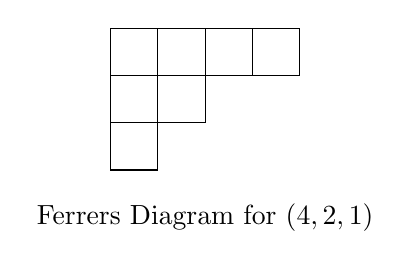
\begin{tikzpicture}[scale=0.6]
  % Ferrers diagram for (4,2,1)
  % Top row: 4 cells (\(\lambda_1=4\))
  \draw (0,0) rectangle (1,1);
  \draw (1,0) rectangle (2,1);
  \draw (2,0) rectangle (3,1);
  \draw (3,0) rectangle (4,1);
  % Second row: 2 cells (\(\lambda_2=2\))
  \draw (0,-1) rectangle (1,0);
  \draw (1,-1) rectangle (2,0);
  % Third row: 1 cell (\(\lambda_3=1\))
  \draw (0,-2) rectangle (1,-1);
  
  \node at (2,-3) {Ferrers Diagram for \((4,2,1)\)};
\end{tikzpicture}
\end{center}

Removing the leftmost column yields:

\begin{center}
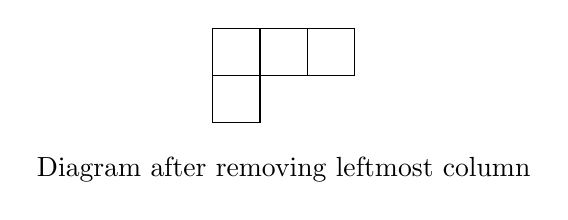
\begin{tikzpicture}[scale=0.6]
  % Diagram after removing the leftmost column from (4,2,1)
  % Top row now has 3 cells
  \draw (0,0) rectangle (1,1);
  \draw (1,0) rectangle (2,1);
  \draw (2,0) rectangle (3,1);
  % Second row now has 1 cell
  \draw (0,-1) rectangle (1,0);
  % Third row now has 0 cells (and is omitted)
  
  \node at (1.5,-2) {Diagram after removing leftmost column};
\end{tikzpicture}
\end{center}

The new diagram represents the partition \((3,1)\), which is a partition of \(7-3=4\) (since there were \(k=3\) rows, and we removed one cell per row). Note that \((3,1)\) is an element of \(P(4,\le 3)\).

\medskip

\textbf{Justification of Bijectivity.}  
The mapping
\[
\Phi\colon (\lambda_1,\lambda_2,\dots,\lambda_k) \mapsto (\lambda_1-1,\lambda_2-1,\dots,\lambda_k-1)
\]
is invertible. Given any partition \(\mu\) in \(P(n-k,\le k)\) (which has at most \(k\) parts), we can reconstruct a unique partition in \(P(n,k)\) by adding \(1\) to each part and, if necessary, appending enough parts equal to \(1\) so that the total number of parts becomes exactly \(k\). In other words, the inverse mapping \(\Phi^{-1}\) is defined by:
\[
\Phi^{-1}\colon \mu = (\mu_1,\mu_2,\dots,\mu_r) \mapsto (\mu_1+1,\mu_2+1,\dots,\mu_r+1,\underbrace{1,1,\dots,1}_{k-r \text{ times}}),
\]
with \(r\le k\). It is straightforward to check that \(\Phi\) and \(\Phi^{-1}\) are mutual inverses. Thus, the mapping \(\Phi\) is a bijection, and we have the relation:
\[
p(n,k)=|P(n,k)| = |P(n-k,\le k)| = p(n-k,\le k).
\]

\medskip

This bijective correspondence is the key step in obtaining a recursive formula for \(p(n,k)\).

\begin{corollary}
For all integers \(n\ge k\ge 1\), we have
\[
p(n,k) = p(n-k,\le k)
      = p(n-k,1) + p(n-k,2) + \cdots + p(n-k,k-1) + p(n-k,k).
\]
That is, the total number of \(k\)-partitions of \(n\) can be split into partitions of \(n-k\) with at most \(k\) parts:
\[
p(n,k) = p(n-k,\le k-1) + p(n-k,k).
\]
Moreover, since
\[
p(n-k,\le k-1)=p((n-k)+(k-1),k-1)=p(n-1,k-1),
\]
we obtain the recurrence relation
\[
p(n,k)=p(n-1,k-1)+p(n-k,k).
\]
\end{corollary}




\section{Inclusion-Exclusion Principle}
\noindent
\textbf{Very often, we need to calculate the number of elements in the union of certain sets.}
Assuming that we know the sizes of these sets, and their mutual intersections, the principle of
inclusion and exclusion allows us to do exactly that.

\medskip

Suppose you have two sets \(A\) and \(B\). The size of the union is certainly at most \(\lvert A\rvert + \lvert B\rvert\). However, in doing so we count each element of \(A \cap B\) twice. To correct for this, we subtract \(\lvert A \cap B\rvert\) to obtain
\[
|A \cup B| \;=\; |A| + |B| \;-\; |A \cap B|.
\]
In general, the formula gets more complicated because we must take into account intersections of multiple sets. The following statement is what we call the \emph{principle of inclusion and exclusion}:

\begin{lemma}
\label{lem:PIE}
For any collection of finite sets \(A_1, A_2, \ldots, A_n\), we have
\[
\left|\bigcup_{i=1}^{n} A_i\right|
\;=\;
\sum_{\substack{I \subseteq [n] \\ I \neq \emptyset}}
(-1)^{\lvert I\rvert + 1}
\left|\bigcap_{i \in I} A_i\right|.
\]
Equivalently,

\[
\resizebox{\textwidth}{!}{$
|A_1 \cup A_2 \cup \cdots \cup A_n|
\;=\;
\sum_{i=1}^n |A_i|
\;-\;
\sum_{1 \le i < j \le n} |A_i \cap A_j|
\;+\;
\sum_{1 \le i < j < k \le n} |A_i \cap A_j \cap A_k|
\;-\;\cdots\;
+\;
(-1)^{n-1}\,\bigl|A_1 \cap A_2 \cap \cdots \cap A_n\bigr|.
$}
\]


\noindent \textbf{Proof Outline (informal):} Each element that belongs to exactly \(t\) of the sets \(A_i\) is counted \(\binom{t}{1}\) times in the first summation, then subtracted \(\binom{t}{2}\) times in the second summation, added \(\binom{t}{3}\) times in the third, and so on. In other words, its total contribution is
\[
\binom{t}{1} - \binom{t}{2} + \binom{t}{3} - \cdots + (-1)^{t-1}\binom{t}{t},
\]
which equals 1. This alternating sum ensures that each element is ultimately counted exactly once, thereby correcting for any overcounting.

\end{lemma}

\section{Permutations and Derangements}

\subsection{Permutations}
A \emph{permutation} of $n$ elements is an arrangement (ordering) of those elements.
For example, there are $6$ permutations of the set $\{a,b,c\}$:
\[
(a,b,c), \quad (a,c,b), \quad (b,a,c), \quad (b,c,a), \quad (c,a,b), \quad (c,b,a).
\]
Since there are $3$ choices for the first element, $2$ for the second (once the first is chosen), and $1$ for the last, by the multiplicative principle there are $3 \cdot 2 \cdot 1 = 3! = 6$ permutations in total.

\paragraph{Factorials and counting.}
In general, the number of permutations of $n$ (distinct) elements is given by
\[
n! \;=\; n \cdot (n-1) \cdot (n-2) \cdots 2 \cdot 1.
\]


\paragraph{Partial permutations (k-permutations).}
Sometimes we only permute $k$ of the $n$ elements, where $1 \le k \le n$. The number of ways to do this is denoted $P(n,k)$ and can be found by thinking:
\[
P(n,k) \;=\; n \times (n-1) \times \cdots \times (n-k+1).
\]
There are $k$ factors in that product. Using factorial notation, we can write
\[
P(n,k) \;=\; \frac{n!}{(n-k)!}.
\]

\paragraph{Relationship to combinations.}
An alternate derivation uses combinations: first \emph{choose} which $k$ elements from the $n$ will appear (that can be done in $\binom{n}{k}$ ways), then \emph{arrange} those $k$ in order (which can be done in $k!$ ways). Hence,
\[
P(n,k) \;=\; \binom{n}{k} \, k!.
\]
Since $\binom{n}{k} = \dfrac{n!}{(n-k)!\,k!}$, multiplying by $k!$ yields exactly $\dfrac{n!}{(n-k)!}$, consistent with the direct counting approach.

\subsection{Derangements}

A \emph{derangement} of $n$ elements is a permutation where no element remains in its original position. More precisely, if we think of a permutation as a bijection $\theta$ on the set $\{1,2,\ldots,n\}$, then $\theta$ is a derangement if and only if 
\[
\theta(k) \;\neq\; k \quad \text{for all } k \in \{1,2,\dots,n\}.
\]
Equivalently, a derangement has no fixed points.

For example, for $n=3$, the permutations of $\{1,2,3\}$ are:
\[
(1,2,3), \quad (1,3,2), \quad (2,1,3), \quad (2,3,1), \quad (3,1,2), \quad (3,2,1).
\]
Among these, the derangements are $(2,3,1)$ and $(3,1,2)$; the other permutations fix at least one of the elements.

\subsubsection*{Counting Derangements via Inclusion-Exclusion}

Let $D(n)$ denote the number of derangements of $n$ elements. We will use the principle of inclusion-exclusion. Suppose we label the elements as $1,2,\dots,n$, and define $A_i$ to be the set of permutations that fix the element~$i$ (i.e.\ $\theta(i)=i$). Then any derangement is a permutation that lies in none of the sets $A_i$ (for $1 \le i \le n$). We have
\[
\bigl|A_i\bigr| \;=\; (n-1)!,
\]
since if we fix one position $i$, then we permute the remaining $n-1$ elements freely. In general,
\[
\bigl|A_{i_1} \cap A_{i_2} \cap \cdots \cap A_{i_k}\bigr| \;=\; (n-k)!.
\]
By inclusion-exclusion, the size of the union $A_1 \cup A_2 \cup \dots \cup A_n$ is
\[
\sum_{k=1}^{n} (-1)^{k+1} \binom{n}{k} (n-k)!.
\]
Hence the number of permutations that do not lie in this union---i.e.\ the number of derangements---is
\[
D(n) \;=\; n! \;-\; \binom{n}{1}(n-1)! + \binom{n}{2}(n-2)! - \cdots + (-1)^n \binom{n}{n}(n-n)!.
\]
\[
D(n) \;=\; \sum_{k=0}^{n} (-1)^k \binom{n}{k} (n-k)!
\;=\; n! \sum_{k=0}^{n} \frac{(-1)^k}{k!}.
\]
Thus, a concise closed-form for the number of derangements is
\[
D(n) \;=\; n!\,\sum_{k=0}^{n} \frac{(-1)^k}{k!}.
\]

\begin{center}
\fbox{%
\parbox{0.9\textwidth}{%
\textbf{Note on the series for \(\boldsymbol{e^{-1}}\):} \\
In Calculus, one learns that the exponential function has a power series expansion
\[
e^x \;=\; \sum_{k=0}^{\infty} \frac{x^k}{k!}.
\]
Setting \(x = -1\) gives
\[
e^{-1} \;=\; \sum_{k=0}^{\infty} \frac{(-1)^k}{k!}.
\]
Hence,
\[
\sum_{k=0}^{n} \frac{(-1)^k}{k!}
\;\xrightarrow[n\to\infty]{}
\; e^{-1}.
\]
If you have not taken (or do not recall) a full course in Calculus, think of this as a special case of a well-known infinite series expansion for the exponential function. 
}%
}
\end{center}

Since the finite sum \(\sum_{k=0}^{n} \frac{(-1)^k}{k!}\) converges to \(e^{-1}\) as \(n \to \infty\), we conclude that
\[
\lim_{n\to\infty} \frac{D(n)}{n!} 
\;=\; \lim_{n\to\infty} 
\sum_{k=0}^{n} \frac{(-1)^k}{k!}
\;=\;
e^{-1}.
\]
Numerically, this means that for large \(n\), about \(1/e \approx 36.8\%\) of all permutations of \(\{1,\dots,n\}\) are derangements (i.e.\ have no fixed points).


\subsubsection*{A Recurrence Relation}
We can also show that $D(n)$ satisfies the recurrence
\[
D(n) \;=\; (n-1)\bigl(D(n-1) + D(n-2)\bigr),
\quad \text{with } D(1)=0, \,D(2)=1.
\]
One way to see this: consider where $1$ goes in a derangement of $\{1,2,\ldots,n\}$. It can go to any of $n-1$ positions. If $1$ goes to position $j$, then either (i)~the element $j$ goes to position $1$ (a swap), which reduces the problem to deranging the remaining $n-2$ elements, or (ii)~the element $j$ does \emph{not} go to position~1, effectively reducing the problem to deranging $n-1$ elements. This yields the above recurrence.

\section{Functions Between Sets}

Let $N$ and $R$ be sets with $|N| = n$ and $|R| = r$.

\begin{enumerate}[label=(\roman*)]
    \item \textbf{Total Functions:}  
    The number of functions from \( N \) to \( R \) is  
    \[
    r^n.
    \]  
    Explanation: For every element in \( N \), there are \( |R| = r \) possible values in \( R \). Thus, for the first element, there are \( r \) choices, for the second element, there are \( r \) choices, and so on.  
    Applying the rule of product, the total number of functions is \( r^n \).

    \item \textbf{Injective Functions:}  
    When \( r \geq n \), an injective function (one-to-one) from \( N \) to \( R \) can be chosen by assigning distinct images to the \( n \) elements.  

    If a function is injective, then for each value in the range there is only one corresponding argument. This means that function values cannot repeat, ensuring that \( x_1 \neq x_2 \) implies \( f(x_1) \neq f(x_2) \).  

    Since there are \( |R| = r \) choices for the first argument, \( r-1 \) choices for the second, \( r-2 \) for the third, and so on, applying the rule of product, the number of injective functions from \( N \) to \( R \) is:  
    \[
    r \cdot (r-1) \cdots (r-n+1) = \frac{r!}{(r-n)!}.
    \]
    \item \textbf{Surjective Functions:}  
    A function is surjective (onto) if every element in \( R \) has a pre-image in \( N \), meaning every element in \( R \) is an image of some element in \( N \).  
    Consider a surjection \( f: N \to R = \{y_1, y_2, \dots, y_r\} \). We observe that the preimages \( f^{-1}(y_1), f^{-1}(y_2), \dots, f^{-1}(y_r) \) form a partition of \( N \) into \( r \) non-empty subsets, as each element \( y_i \) in \( R \) corresponds to one or more elements from \( N \).  
    The number of ways to partition \( N \) into \( r \) parts is given by the Stirling number \( S(n, r) \), and since we can permute the \( r \) elements in \( R \) in \( r! \) ways, the total number of surjective functions from \( N \) to \( R \) is:  
    \[
    r! \, S(n, r),
    \]
    where \( S(n, r) \) is the Stirling number of the second kind, counting the ways to partition \( N \) into \( r \) non-empty subsets.

\end{enumerate}

\paragraph{Example:}  
For \( N = \{1, 2, 3\} \) and \( R = \{y_1, y_2\} \):
\begin{itemize}[nosep]
    \item[] Here \( |N| = 3 \) and \( |R| = 2 \).
    \item Total functions: $2^3 = 8$.
    \item Injective functions: Not possible since $|R|<|N|$.
    \item Surjective functions: Consider all possible surjective functions:

 \( f_1: \{1, 2\} \mapsto y_1, 3 \mapsto y_2 \)
- Another possible permutation for this partition: \( f_2: \{1, 2\} \mapsto y_2, 3 \mapsto y_1 \)
 \( f_3: \{2, 3\} \mapsto y_1, 1 \mapsto y_2 \)
- Another possible permutation for this partition: \( f_4: 1 \mapsto y_1, \{2, 3\} \mapsto y_2 \)
 \( f_5: \{1, 3\} \mapsto y_1, 2 \mapsto y_2 \)
- Another possible permutation for this partition: \( f_6: 2 \mapsto y_1, \{1, 3\} \mapsto y_2 \)

So, we have 6 surjective functions. Using the formula for surjective functions, we first find the Stirling number \( S(3, 2) = 3 \), which corresponds to the number of partitions without considering permutations. Then, accounting for the permutations of the \( r = 2 \) elements in \( R \), we compute:
\[
2! \cdot S(3, 2) = 2! \cdot 3 = 6,
\]
which matches the number of surjective functions we listed.
\end{itemize}

\section{Generating functions}
\subsection*{Generating Series}

Instead of viewing a sequence as a function that returns its \(n\)th term, a \emph{generating series} packages all of its terms into a single power series whose coefficients are exactly the sequence entries.  Concretely, the sequence
\[
2,\;3,\;5,\;8,\;12,\;\dots
\]
is encoded by the generating series
\[
2 + 3x + 5x^2 + 8x^3 + 12x^4 + \cdots.
\]

In general, given any sequence \(\{c_n\}_{n\ge0}\), its generating series is the formal power series

\[
G(x) \;=\; \sum_{n=0}^\infty c_n x^n 
\;=\;
c_0 + c_1 x + c_2 x^2 + c_3 x^3 + \cdots.
\]

We say that \(G(x)\) “generates” the sequence \(\{c_n\}\) because each coefficient of \(x^n\) in \(G(x)\) is precisely \(c_n\).  Generating series turn sequence‑based problems into algebraic manipulations of power series, a technique we will exploit heavily in what follows.

\subsection*{Recall of the Basic Series}
\paragraph{A Geometric View of the Binary Series}
\begin{figure}[ht]
  \centering
  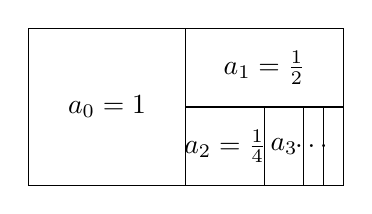
\begin{tikzpicture}[scale=2]
      % Draw outer rectangle (width=2, height=1)
      \draw (0,0) rectangle (2,1);
  
      % Partition line between a0 and the rest
      \draw (1,0) -- (1,1);
  
      % Label a0
      \node at (0.5,0.5) {$a_0 = 1$};
  
      % Horizontal partition for the right half (top sub-rectangle a1)
      \draw (1,0.5) -- (2,0.5);
      \node at (1.5,0.75) {$a_1 = \frac{1}{2}$};
  
      % Vertical partition for the bottom half (a2, a3, ...)
      \draw (1.5,0) -- (1.5,0.5);
      \node at (1.25,0.25) {$a_2 = \frac{1}{4}$};
  
      % Subdivide further for illustration (a3, a4, …)
      \draw (1.75,0) -- (1.75,0.5);
      \draw (1.875,0) -- (1.875,0.5);
  
      % Place a3 label (you can add more if you like)
      \node at (1.625,0.25) {$a_3$};
      \node at (1.8125,0.25) {$\dots$};
\end{tikzpicture}
\caption{A geometric interpretation of the binary series, showing how 
\(\sum_{n=0}^{\infty} \tfrac{1}{2^n} = 2\).}
\end{figure}
For \(|x| < 1\), we have the infinite geometric series
\[
\frac{1}{1-x} = 1 + x + x^2 + x^3 + \cdots = \sum_{n=0}^{\infty} x^n.
\]
We now present a quick proof of this result by performing long division of \(1\) by \(1-x\).

\[
\renewcommand{\arraystretch}{1.3}
\begin{array}{r|l}
 & 1 + x + x^2 + x^3 + \cdots \\ % quotient
1 - x & 1  \\ % divisor | dividend
\hline
 & \underline{1 - x} \\
 & x \\
 & \underline{x - x^2} \\
 & x^2 \\
 & \underline{x^2 - x^3} \\
 & x^3 \\
 & \vdots
\end{array}
\]


The process works as follows:
The long‑division proceeds by repeatedly dividing the current remainder by the leading term of the divisor, producing one new power of \(x\) at each step:

\begin{enumerate}
  \item Divide \(1\) by \(1-x\). The multiplier needed to eliminate the constant term is \(1\), so 
  \[
    1 - 1\cdot(1-x) = x.
  \]
  Thus the first summand is \(1\), leaving a remainder of \(x\).

  \item Divide the remainder \(x\) by \(1-x\). The multiplier is \(x\), so
  \[
    x - x\cdot(1-x) = x^2.
  \]
  Hence the second summand is \(x\), leaving a remainder of \(x^2\).

  \item Divide \(x^2\) by \(1-x\). The multiplier is \(x^2\), giving
  \[
    x^2 - x^2\cdot(1-x) = x^3.
  \]
  Therefore the third summand is \(x^2\), with remainder \(x^3\).

  \item Continuing in this fashion produces the infinite series
  \[
    \frac{1}{1-x} = 1 + x + x^2 + x^3 + \cdots.
  \]
\end{enumerate}


Continuing indefinitely produces
\[
\frac{1}{1-x} = 1 + x + x^2 + x^3 + \cdots = \sum_{n=0}^\infty x^n,
\]
as claimed. \par
\noindent We will use this fact in further examples throughout the notes.

\subsection{Building Generating Functions}

The simplest (or “basic”) generating function is
\[
\frac{1}{1-x} = 1 + x + x^2 + x^3 + \cdots,
\]
which generates the constant sequence \(1,1,1,\dots\).

\medskip
\noindent
\textbf{Replacing \(x\) with \(-x\):}
\[
\frac{1}{1-(-x)} = \frac{1}{1+x} = 1 - x + x^2 - x^3 + \cdots,
\]
generating \(1,-1,1,-1,\dots\).

\medskip
\noindent
\textbf{Replacing \(x\) with \(3x\):}
\[
\frac{1}{1-3x} = 1 + 3x + 9x^2 + 27x^3 + \cdots,
\]
generating \(1,3,9,27,\dots\).

\medskip
\noindent
\textbf{Scaling a sequence by 3:}
\[
\frac{3}{1-3x} = 3 + 9x + 27x^2 + 81x^3 + \cdots,
\]
generating \(3,9,27,81,\dots\).

\medskip
\noindent
\textbf{Termwise addition of sequences:}\\
Adding the generating functions for \(1,1,1,\dots\) and \(1,3,9,\dots\) gives
\[
\frac{1}{1-x} + \frac{1}{1-3x}
= 2 + 4x + 10x^2 + 28x^3 + \cdots,
\]
which generates \(2,4,10,28,\dots\).

\medskip
\noindent
\textbf{Replacing \(x\) with \(x^2\):}
\[
\frac{1}{1-x^2} = 1 + x^2 + x^4 + x^6 + \cdots,
\]
generating \(1,0,1,0,1,0,\dots\).

\medskip
\noindent
\textbf{Shifting a sequence:}\\
Multiplying by \(x\) shifts all coefficients right by one:
\[
\frac{x}{1-3x} = 0 + x + 3x^2 + 9x^3 + \cdots,
\]
generating \(0,1,3,9,\dots\), and
\[
\frac{x}{1-x^2} = 0 + x + 0x^2 + x^3 + \cdots,
\]
generating \(0,1,0,1,\dots\).

\medskip
\noindent
\textbf{Combining shifted sequences:}\\
Adding the two “even‑odd” generating functions recovers
\[
\frac{1}{1-x^2} + \frac{x}{1-x^2} = \frac{1+x}{1-x^2} = \frac{1}{1-x},
\]
which generates \(1,1,1,1,\dots\).

\medskip
\noindent
\textbf{Differentiation:}\\
Differentiating the basic Generating Function
\[
\frac{d}{dx}\!\Bigl(\frac{1}{1-x}\Bigr)
= \frac{1}{(1-x)^2}
= 1 + 2x + 3x^2 + 4x^3 + \cdots,
\]
yields the generating function for \(1,2,3,4,\dots\).


\medskip

\FloatBarrier            % ensure the Differentiation figure/text finishes here

\subsection{Recurrence Relations \& Generating Functions}

We conclude with an example of one of the many reasons studying generating functions is helpful: solving recurrence relations via algebraic manipulation of power series.

\paragraph{Example: Tower of Hanoi}  
The minimum number of moves required to transfer \(n\) disks satisfies
\[
a_0 = 0,\quad
a_1 = 1,\quad
a_n = 2\,a_{n-1} + 1 \quad(n\ge1),
\]
giving the sequence
\[
0,\;1,\;3,\;7,\;15,\;31,\dots
\]

\begin{figure}[ht]
  \centering
  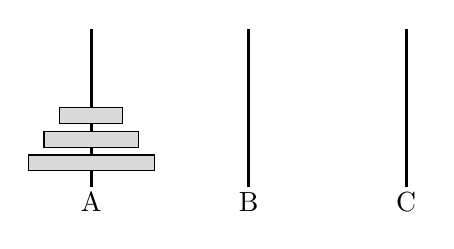
\begin{tikzpicture}[scale=1]
    % Draw three pegs
    \foreach \x in {0,2,4} {
      \draw[line width=1pt] (\x,0) -- (\x,2);
    }
    % Draw disks on left peg
    \foreach \i/\w in {0.2/1.6,0.5/1.2,0.8/0.8} {
      \draw[fill=gray!30] (0-\w/2,\i) rectangle (0+\w/2,\i+0.2);
    }
    \node at (0,-0.2) {A};
    \node at (2,-0.2) {B};
    \node at (4,-0.2) {C};
  \end{tikzpicture}
  \caption{Initial configuration for Tower of Hanoi (3 disks).}
\end{figure}

Define the generating function
\[
f(x) = \sum_{n=0}^\infty a_n x^n.
\]
Using the recurrence for \(n\ge1\):
\[
\sum_{n=1}^\infty a_n x^n 
= \sum_{n=1}^\infty \bigl(2a_{n-1}+1\bigr)x^n
= 2x\sum_{n=0}^\infty a_n x^n + \sum_{n=1}^\infty x^n,
\]
so
\[
f(x) - a_0 = 2x\,f(x) + \frac{x}{1-x},
\]
and since \(a_0=0\),
\[
f(x) = \frac{x}{(1-x)(1-2x)}.
\]

Performing partial fractions:
\[
\frac{x}{(1-x)(1-2x)}
= \frac{-1}{1-x} + \frac{1}{1-2x},
\]
hence
\[
f(x) = -\frac{1}{1-x} + \frac{1}{1-2x}.
\]

Extracting coefficients yields the closed‑form solution
\[
a_n = 2^n - 1,
\]
confirming the well‑known formula for the Tower of Hanoi moves.
\FloatBarrier

\subsection{Introduction to the Fibonacci Sequence}
The Fibonacci sequence famously arises from a puzzle involving rabbit populations.
Imagine starting with a single pair of rabbits that takes one month to mature.
After maturing, each pair produces a new pair of rabbits every month.
Mathematically, if \(F_n\) represents the number of rabbit pairs in month \(n\),
the sequence satisfies the initial conditions
\[
F_0 = 0, \quad F_1 = 1,
\]
and the recurrence
\[
F_{n+2} = F_{n+1} + F_n \quad \text{for} \; n \ge 0.
\]

\begin{figure}[ht]
  \centering
  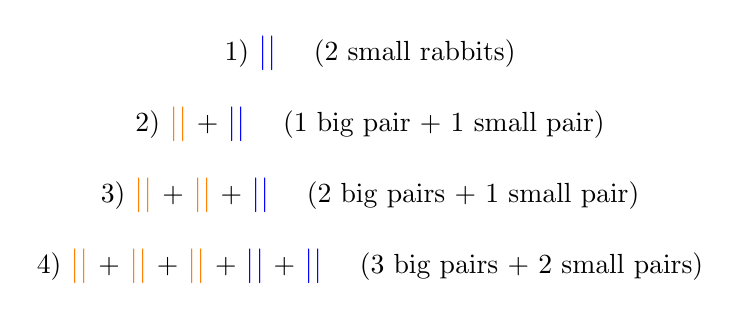
\begin{tikzpicture}[x=1cm, y=0.9cm]
      % Month 1
      \node at (0,0) {1) \(\textcolor{blue}{\big|\big|}\) \quad (2 small rabbits)};
      % Month 2
      \node at (0,-1) {2) \(\textcolor{orange}{\big|\big|}\) + \(\textcolor{blue}{\big|\big|}\) 
        \quad (1 big pair + 1 small pair)};
      % Month 3
      \node at (0,-2) {3) \(\textcolor{orange}{\big|\big|}\) + \(\textcolor{orange}{\big|\big|}\) + \(\textcolor{blue}{\big|\big|}\)
        \quad (2 big pairs + 1 small pair)};
      % Month 4
      \node at (0,-3) {4) \(\textcolor{orange}{\big|\big|}\) + \(\textcolor{orange}{\big|\big|}\) + \(\textcolor{orange}{\big|\big|}\) 
        + \(\textcolor{blue}{\big|\big|}\) + \(\textcolor{blue}{\big|\big|}\)
        \quad (3 big pairs + 2 small pairs)};
\end{tikzpicture}
\caption{Illustration of rabbit pairs over successive months. 
Blue bars represent small rabbits; orange bars represent big (mature) rabbits.}
\end{figure}

Q: is there a non-recursive (closed-form) formula for \(F_n\) ?
\paragraph{Idea: consider and calculate it}

\subsection{Deriving the Closed-Form for the Fibonacci Sequence}

\paragraph{Step 1: Define the generating function.}
Let \(\{F_n\}_{n=0}^{\infty}\) be the Fibonacci sequence with 
\[
F_0 = 0, \quad F_1 = 1, \quad F_{n+2} = F_{n+1} + F_n \quad (n \ge 0).
\]
Define the generating function
\[
f(x) \;=\; \sum_{n=0}^{\infty} F_n\,x^n.
\]
We aim to find a closed-form expression for \(f(x)\), and then extract a formula for \(F_n\).

\paragraph{Step 2: Use the Fibonacci recurrence in \(f(x)\).}
Starting from
\[
f(x) \;=\; F_0 + F_1 x + \sum_{n=2}^{\infty} F_n\,x^n,
\]
and noting \(F_0=0\), \(F_1=1\), we have
\[
f(x) \;=\; x + \sum_{n=2}^{\infty} \bigl(F_{n-1} + F_{n-2}\bigr)\,x^n
\]
because \(F_n = F_{n-1} + F_{n-2}\) for \(n\ge2\). Separate the sums:
\[
f(x)
= x
+ \sum_{n=2}^{\infty} F_{n-1}\,x^n
+ \sum_{n=2}^{\infty} F_{n-2}\,x^n.
\]
Shift indices to factor out \(f(x)\):
\[
\sum_{n=2}^{\infty} F_{n-1}\,x^n 
= x \sum_{n=2}^{\infty} F_{n-1}\,x^{n-1} 
= x \sum_{m=1}^{\infty} F_m\,x^m 
= x \bigl(f(x) - F_0\bigr) 
= x\,f(x),
\]
since \(F_0=0\). Similarly,
\[
\sum_{n=2}^{\infty} F_{n-2}\,x^n 
= x^2 \sum_{n=2}^{\infty} F_{n-2}\,x^{n-2}
= x^2 \sum_{k=0}^{\infty} F_k\,x^k
= x^2\,f(x).
\]
Hence,
\[
f(x) = x + x\,f(x) + x^2\,f(x) 
\;\;\Longrightarrow\;\;
f(x)\bigl(1 - x - x^2\bigr) = x.
\]
Thus,
\[
f(x) = \frac{x}{\,1 - x - x^2\,}.
\]

\paragraph{Step 3: Partial-Fraction Decomposition (as in the images).}

First, rewrite
\[
\frac{1}{1 - x - x^2}
\;=\;
\frac{1}{-\bigl(x^2 + x - 1\bigr)}
\;=\;
-\,\frac{1}{x^2 + x - 1}.
\]

\noindent
Next, factor \(x^2 + x - 1\). Observe that the roots of
\[
x^2 + x - 1 \;=\; 0
\]
are
\[
x \;=\; -\,\frac{1 + \sqrt{5}}{2}
\quad\text{and}\quad
x \;=\; -\,\frac{1 - \sqrt{5}}{2}.
\]
Hence,
\[
x^2 + x - 1
\;=\;
\Bigl(x + \tfrac{1 + \sqrt{5}}{2}\Bigr)
\;\cdot\;
\Bigl(x + \tfrac{1 - \sqrt{5}}{2}\Bigr).
\]
Therefore,
\[
-\,\frac{1}{x^2 + x - 1}
\;=\;
-\,\frac{1}{\Bigl(x + \tfrac{1 + \sqrt{5}}{2}\Bigr)\,\Bigl(x + \tfrac{1 - \sqrt{5}}{2}\Bigr)}.
\]
We look for constants \(A\) and \(B\) such that
\[
-\,\frac{1}{\Bigl(x + \tfrac{1 + \sqrt{5}}{2}\Bigr)\,\Bigl(x + \tfrac{1 - \sqrt{5}}{2}\Bigr)}
\;=\;
\frac{A}{\,x + \tfrac{1 + \sqrt{5}}{2}\,}
\;+\;
\frac{B}{\,x + \tfrac{1 - \sqrt{5}}{2}\,}.
\]


\paragraph{Step 4: Solve for \(A\) and \(B\).}

Comparing coefficients of \(x\) and the constant term in
\[
-\,1
\;=\;
A\Bigl(x + \beta\Bigr)
\;+\;
B\Bigl(x + \alpha\Bigr),
\]
we obtain the system
\[
\begin{cases}
A + B = 0, \\[4pt]
A\,\beta + B\,\alpha = -\,1.
\end{cases}
\]
It follows that
\[
B = -\,A,
\quad
A\,(\beta - \alpha) = -\,1
\;\;\Longrightarrow\;\;
A = \frac{1}{\alpha - \beta}
\quad\text{and}\quad
B = -\,\frac{1}{\alpha - \beta}.
\]
Hence,
\[
-\,\frac{1}{(x+\alpha)(x+\beta)}
\;=\;
\frac{1}{\alpha - \beta}\,\frac{1}{\,x+\alpha\,}
\;-\;
\frac{1}{\alpha - \beta}\,\frac{1}{\,x+\beta\,}.
\]

\paragraph{Step 5: Combine with the earlier factor \(-1\) and rewrite.}

Recalling that
\[
\frac{1}{1 - x - x^2}
\;=\;
-\,\frac{1}{\,x^2 + x - 1\,}
\;=\;
-\,\frac{1}{\,(x+\alpha)\,(x+\beta)\,},
\]
we combine the above result to conclude
\[
\frac{1}{1 - x - x^2}
\;=\;
\frac{1}{\alpha - \beta}
\left(
\frac{1}{\,x+\alpha\,}
\;-\;
\frac{1}{\,x+\beta\,}
\right).
\]

\paragraph{Step 6: Expand each term in a power series.}

Notice that
\[
\frac{1}{x + \alpha}
\;=\;
\frac{1}{\alpha}\,\frac{1}{1 + \tfrac{x}{\alpha}}
\;=\;
\frac{1}{\alpha}\,\sum_{n=0}^\infty \bigl(-\tfrac{x}{\alpha}\bigr)^{n}
\;=\;
\sum_{n=0}^\infty
\frac{(-1)^n}{\,\alpha^{\,n+1}\!}\,
x^n,
\]
valid for \(\bigl|\tfrac{x}{\alpha}\bigr| < 1\).  Similarly,
\[
\frac{1}{x + \beta}
\;=\;
\sum_{n=0}^\infty
\frac{(-1)^n}{\,\beta^{\,n+1}\!}\,
x^n.
\]
Hence,
\[
\frac{1}{1 - x - x^2}
\;=\;
\frac{1}{\alpha - \beta}
\left[
\sum_{n=0}^\infty \frac{(-1)^n}{\,\alpha^{\,n+1}\!}\,x^n
\;-\;
\sum_{n=0}^\infty \frac{(-1)^n}{\,\beta^{\,n+1}\!}\,x^n
\right]
=
\sum_{n=0}^\infty
\left[
\frac{1}{\alpha - \beta}
\Bigl(
\frac{(-1)^n}{\,\alpha^{\,n+1}\!}
\;-\;
\frac{(-1)^n}{\,\beta^{\,n+1}\!}
\Bigr)
\right]
x^n.
\]

\paragraph{Step 7: Identify Fibonacci numbers.}

Recall that \(\alpha - \beta = \sqrt{5}\), and
\[
F_n
\;=\;
\frac{\alpha^n - \beta^n}{\,\alpha - \beta\,}
\;=\;
\frac{\alpha^n - \beta^n}{\,\sqrt{5}\,}.
\]
One checks (or uses known identities) to see that the coefficient of \(x^n\) in the above power series is exactly \(F_n\).  Consequently,
\[
\sum_{n=0}^\infty F_n \, x^n
\;=\;
\frac{1}{\,1 - x - x^2\,},
\]
which is the generating function for the Fibonacci sequence.

\paragraph{Conclusion.}
We have shown that the generating function for the Fibonacci sequence is 
\(\tfrac{x}{1 - x - x^2}\).  
Through partial fractions and comparing coefficients, we deduced that
\[
F_n = \frac{\alpha^n - \beta^n}{\sqrt{5}}.
\]
This gives a non-recursive (closed-form) expression for \(F_n\), completing the derivation.

\subsection{More examples}

In earlier sections (see, e.g., \emph{A Geometric View of the Binary Series} on page~14), we explored methods to solve recurrences and introduced generating functions as a tool to transform sequences into functions. In this section, we briefly reiterate these ideas and demonstrate, through several examples, how generating functions serve as a bridge between discrete mathematics and calculus.

\paragraph{Example 1: Constant Sequence.}  
Consider the sequence defined by
\[
a_n=1 \quad \text{for all } n\ge0,
\]
so that the sequence is
\[
1,\,1,\,1,\dots.
\]
By the geometric series formula (proved earlier), its generating function is given by
\[
f(x)=\sum_{n=0}^{\infty} x^n=\frac{1}{1-x}, \quad |x|<1.
\]

\paragraph{Example 2: Exponential Sequence.}  
Now, let
\[
a_n=\frac{1}{n!}.
\]
Then the generating function is
\[
f(x)=\sum_{n=0}^{\infty} \frac{x^n}{n!}=e^x, \quad x\in\mathbb{R}.
\]
A partial justification of this result can be obtained by recalling the Taylor series expansion of the exponential function. Although a complete treatment of Taylor series is a topic in calculus (not yet covered in this course), note that differentiating the power series term-by-term confirms the identity.

\paragraph{Example 3: Binomial Coefficient Sequence.}  
Consider the sequence defined by
\[
a_n=\binom{n+k}{k}.
\]
\textbf{Theorem.} The generating function for this sequence is
\[
f(x)=\sum_{n=0}^{\infty}\binom{n+k}{k}x^n=\frac{1}{(1-x)^{k+1}}, \quad |x|<1.
\]
\newpage
\textit{Proof.}  
\begin{itemize}
    \item For \(k=1\): Note that
    \[
    \ a_n = \binom{n+1}{1} = n+1,
    \]
    so that
    \[
    f(x) = \sum_{n=0}^{\infty} \binom{n+1}{1} x^n = \sum_{n=0}^{\infty} (n+1)x^n.
    \]
    Recall the geometric series,
    \[
    \frac{1}{1-x} = \sum_{n=0}^{\infty} x^n,
    \]
    and observe that by differentiating both sides term-by-term with respect to \(x\), we can derive the generating function for the sequence \((n+1)\). In detail, differentiate the left-hand side:
    \[
    \frac{d}{dx}\left(\frac{1}{1-x}\right) = \frac{1}{(1-x)^2}.
    \]
    On the right-hand side, notice that since
    \[
    \frac{d}{dx}\,x^{n+1} = (n+1)x^n,
    \]
    differentiating the series yields
    \[
    \frac{d}{dx}\left(\sum_{n=0}^{\infty} x^n\right) = \sum_{n=0}^{\infty} (n+1)x^n.
    \]
    Thus, we conclude that
    \[
    \frac{1}{(1-x)^2} = \sum_{n=0}^{\infty} (n+1)x^n.
    \]
    This recovers the generating function for \(k=1\). A less formal derivation was given in the subsection \emph{Building Generating Functions} on page~16.
\end{itemize}
A complete inductive proof follows similar lines but is omitted here for brevity.

\paragraph{Example 4: Alternating Factorial Sequence.}  
Define the sequence by
\[
a_n=
\begin{cases}
0, & \text{if } n \text{ is even},\\[1mm]
\displaystyle \frac{(-1)^{\frac{n-1}{2}}}{n!}, & \text{if } n \text{ is odd}.
\end{cases}
\]
Then the generating function is
\[
f(x)=x-\frac{x^3}{3!}+\frac{x^5}{5!}-\frac{x^7}{7!}+\cdots=\sin(x), \quad x\in\mathbb{R}.
\]
Even though a full treatment of the Taylor series for trigonometric functions is part of calculus (again, a topic not yet covered here), this example illustrates how generating functions capture nontrivial sequence behavior by connecting discrete structures with analytic functions.

\subsection{Generating Function Applications}

One key application is the multiplication (or convolution) of generating functions, which naturally arises when we combine two distinct combinatorial constructions into a single, more complex structure.

\textbf{Question:} If \(a_k\) counts all objects of type A of size \(k\) and \(b_k\) counts all objects of type B of size \(k\), how many pairs of objects \((A, B)\) have a total size of \(n\)?

\textbf{Answer:} The number of such pairs is given by
\[
\sum_{k=0}^{n} a_k\, b_{n-k}.
\]

\textbf{Observation:} The generating function for the sequence
\[
C_n = \sum_{k=0}^{n} a_k\, b_{n-k}
\]
is
\[
\sum_{n=0}^{\infty} C_n\, x^n = \sum_{n=0}^{\infty} \left(\sum_{k=0}^{n} a_k\, b_{n-k}\right)x^n.
\]
It shows that multiplying the generating functions corresponding to \( \{a_n\} \) and \( \{b_n\} \) produces a new generating function whose coefficients are given by the convolution of the two original sequences.


\paragraph{Example: Dice Sum Counting.}  
A classic example of this application is counting the number of ways to obtain a given sum when rolling two standard six-sided dice. For a single die, the generating function is:
\[
D(x) = x + x^2 + x^3 + x^4 + x^5 + x^6,
\]
where the term \(x^k\) corresponds to rolling a \(k\). Since the two dice are independent, the generating function for the sum of the two dice is:
\[
D(x)^2 = \left(x + x^2 + x^3 + x^4 + x^5 + x^6\right)^2.
\]
Expanding this product, the coefficient of \(x^n\) in \(D(x)^2\) equals the number of ways to achieve a total sum of \(n\). For instance, one can verify that the coefficient of \(x^7\) is 6, which corresponds to the six possible outcomes that sum to 7 (namely, the pairs \((1,6), (2,5), (3,4), (4,3), (5,2), (6,1)\)).

\section{Catalan Numbers}
\subsection{Introduction and Motivating Problem}

How many ways can we correctly place $n$ pairs of parentheses? This is a classic combinatorial question about **valid parentheses combinations**. For example, with $n=1$ pair, there is only one valid arrangement: `()`. With $n=2$ pairs, there are two valid arrangements: `()()` and `(())`. With $n=3$ pairs, there are five valid arrangements (e.g. `()()()`, `()(())`, `(())()`, `(()())`, `((()))`). In general, the number of distinct well-formed parentheses sequences grows quickly with $n$. 

This problem was our motivation to study a famous sequence of numbers. (It has connection to a similar LeetCode programming problem about generating parentheses.) The numbers counting valid parentheses structures for $n=1,2,3,\dots$ are:

\[1,\; 2,\; 5,\; 14,\; 42,\; 132,\;\dots\]

These are known as the **Catalan numbers**. In these notes, we will explore Catalan numbers, their recursive definition, how they relate to binary tree structures, and a derivation of their formula using generating functions.

\subsection{Definition of Catalan Numbers}

The Catalan numbers $C_n$ can be defined recursively. For $n=0$ (zero pairs of parentheses), we define $C_0 = 1$ by convention (there is exactly one valid arrangement of zero pairs: an empty sequence). For $n\ge 1$, the Catalan number $C_n$ satisfies the recursion:

\[
C_n \;=\; \sum_{k=0}^{\,n-1} C_k \;\cdot\; C_{\,n-1-k}\,.
\]

In other words, each $C_n$ is obtained by summing over all products $C_k \cdot C_{n-1-k}$ for $0 \le k \le n-1$. This recurrence is the heart of what makes Catalan numbers arise in so many combinatorial structures. We will soon see why this recurrence formula makes sense in terms of counting valid parentheses or binary tree configurations.

\textit{*(Additional note: There is also a direct formula for $C_n$ which we will derive later. The first few values $C_0=1$, $C_1=1$, $C_2=2$, $C_3=5$, $C_4=14$ confirm the sequence given above.)*}

\subsection*{Combinatorial reasoning (parenthesis perspective)}

Why does the above recurrence hold for valid parentheses? Consider a valid parentheses sequence of $n$ pairs. Focus on the very first “(`” character. It must have a matching “)`”. Say this matching “)`” occurs after forming $k$ pairs inside (between this “(`” and its matching “)`”) – those $k$ pairs inside must themselves form a valid sequence. The remaining parentheses (after the matching “)`”) will form another valid sequence with $n-1-k$ pairs. See the schematic below for a sequence split by the first pair:

\[
\underbrace{\vphantom{()}( \;\;\; S_{\text{inside}} \;\;\; )}_{\text{$1+k$ pairs}} \;\; S_{\text{outside}}\,,
\] 

where $S_{\text{inside}}$ is a valid sequence of $k$ pairs, and $S_{\text{outside}}$ is a valid sequence of $n-1-k$ pairs. Any valid sequence can be uniquely decomposed in this way. There are $C_k$ possibilities for $S_{\text{inside}}$ and $C_{\,n-1-k}$ possibilities for $S_{\text{outside}}$. Multiplying and summing over all $k$ from $0$ to $n-1$ gives the recurrence $C_n = \sum_{k=0}^{n-1} C_k\,C_{n-1-k}$, as stated above.

\textit{*(Additional note: The same recurrence will be explained again using binary trees below, which is an equivalent interpretation. The key idea is splitting a structure (parentheses or tree) at a certain point, resulting in two smaller independent structures.)*}

\subsection{Catalan Numbers and Binary Trees}

Catalan numbers also count the number of distinct **binary tree** structures with a given number of nodes. To appreciate this connection, we first review what a binary tree is:

A **binary tree** is a hierarchical structure consisting of nodes, where each node may have up to two children: a left child and a right child. A node with no children is called a *leaf*. We often draw binary trees in a planar way with the root at the top, left children branching to the left, and right children to the right. In counting binary trees for Catalan numbers, we consider different shapes of the tree (different arrangements of nodes and child connections) as distinct, but we do *not* label the nodes with any specific values.

For example, with only 1 node, there is exactly one possible binary tree (just the root by itself). With 2 nodes, there are exactly two distinct binary tree shapes:

\begin{center}
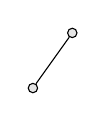
\begin{tikzpicture}[level distance=7mm, sibling distance=10mm, every node/.style={circle, draw, fill=black!10, inner sep=1.2pt}]
\node {} 
  child { node {} }
  child[missing] {};
\end{tikzpicture}
\hspace{1cm}
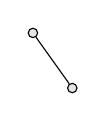
\begin{tikzpicture}[level distance=7mm, sibling distance=10mm, every node/.style={circle, draw, fill=black!10, inner sep=1.2pt}]
\node {}
  child[missing] {} 
  child { node {} };
\end{tikzpicture}
\end{center}

In the first tree above, the root has a left child but no right child. In the second tree, the root has a right child but no left child. These are the only two possible configurations for 2 nodes. Now, for 3 nodes, it turns out there are 5 distinct binary tree shapes. We can enumerate all five (to visualize them, each diagram below shows the shape, with nodes represented by circles):

\begin{center}
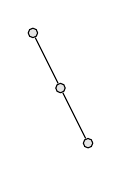
\begin{tikzpicture}[baseline=-2pt, level distance=7mm, sibling distance=7mm, every node/.style={circle, draw, fill=black!10, inner sep=1.2pt}]
\node {} 
  child[missing] {} 
  child { node {} 
            child[missing] {} 
            child { node {} } };
\end{tikzpicture}
\hfill
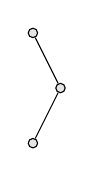
\begin{tikzpicture}[baseline=-2pt, level distance=7mm, sibling distance=7mm, every node/.style={circle, draw, fill=black!10, inner sep=1.2pt}]
\node {}
  child[missing] {} 
  child { node {}
            child { node {} } 
            child[missing] {} };
\end{tikzpicture}
\hfill
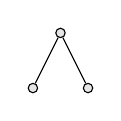
\begin{tikzpicture}[baseline=-2pt, level distance=7mm, sibling distance=7mm, every node/.style={circle, draw, fill=black!10, inner sep=1.2pt}]
\node {} 
  child { node {} }
  child { node {} };
\end{tikzpicture}
\hfill
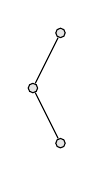
\begin{tikzpicture}[baseline=-2pt, level distance=7mm, sibling distance=7mm, every node/.style={circle, draw, fill=black!10, inner sep=1.2pt}]
\node {}
  child { node {}
            child[missing] {} 
            child { node {} } }
  child[missing] {};
\end{tikzpicture}
\hfill
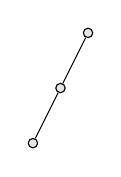
\begin{tikzpicture}[baseline=-2pt, level distance=7mm, sibling distance=7mm, every node/.style={circle, draw, fill=black!10, inner sep=1.2pt}]
\node {}
  child { node {}
            child { node {} } 
            child[missing] {} }
  child[missing] {};
\end{tikzpicture}
\end{center}

\vspace{1ex}
\begin{center}
\small (All 5 distinct binary trees with 3 nodes)
\end{center}
\vspace{1ex}

For 3 nodes, the five tree shapes can be described as:
1. A right-skewed chain (root $\to$ right child $\to$ right grandchild).
2. A tree where the root has only a right child, and that child in turn has a left child.
3. A balanced tree (root with one left child and one right child).
4. A tree where the root has only a left child, and that child has a right child.
5. A left-skewed chain (root $\to$ left child $\to$ left grandchild).

If we proceed to 4 nodes, the number of distinct binary trees grows to 14. Detailing all 14 shapes is cumbersome, but we can categorize them by how the root splits the nodes between left and right subtrees:
- 5 of those trees have all 3 of the other nodes in the left subtree (and right subtree empty), and another 5 have all 3 in the right subtree (left empty). These 10 are essentially a root with one side empty and the other side being one of the 5 shapes from the 3-node case.
- 2 of the trees have the root with 1 node in the left subtree and 2 in the right subtree.
- The remaining 2 have 2 nodes in the left subtree and 1 in the right subtree.

Adding these cases: $5 + 5 + 2 + 2 = 14$ total shapes for 4 nodes. (Indeed, 14 is the next Catalan number after 5.)

This pattern is no coincidence. In fact, the recurrence relation for $C_n$ can be understood by considering how a binary tree of $n$ nodes can be formed. Suppose a binary tree has $n$ nodes in total. Pick a number $k$ between $0$ and $n-1$ (inclusive) to be the number of nodes in the left subtree of the root. Then the right subtree will have $n-1-k$ nodes (since one node is the root itself). There are $C_k$ possible shapes for the left subtree (by definition of Catalan numbers for $k$ nodes) and $C_{\,n-1-k}$ possible shapes for the right subtree. These choices are independent, so there are $C_k \cdot C_{\,n-1-k}$ possible trees with that particular split of $k$ and $n-1-k$. Summing over all $k=0,1,2,\dots,n-1$ gives exactly $C_n = \sum_{k=0}^{n-1} C_k\,C_{n-1-k}$. This is the same recursive formula we encountered earlier, now interpreted in terms of binary trees. Thus, the number of valid parentheses arrangements with $n$ pairs is equal to the number of binary tree structures with $n$ nodes, and both are given by the $n$th Catalan number.

\subsection{Deriving the Formula using Generating Functions}

While the recursive definition of Catalan numbers is useful, we can go further and derive a closed-form formula for $C_n$. A powerful method to solve such recurrences is to use a **generating function**. Define the generating function $C(x)$ for the Catalan sequence as:

\[
C(x) \;=\; C_0 + C_1 x + C_2 x^2 + C_3 x^3 + \cdots \;=\; \sum_{n\ge 0} C_n \, x^n\,.
\]

Using the recurrence $C_n = \sum_{k=0}^{n-1} C_k\,C_{n-1-k}$, we can derive an equation for $C(x)$. First, note that:

\[
C(x) - C_0 \;=\; \sum_{n\ge 1} C_n x^n \;=\; \sum_{n\ge 1}\Big(\sum_{k=0}^{n-1} C_k\,C_{n-1-k}\Big) x^n\,.
\]

Now, change the summation index by letting $m = n-1$. Then $n\ge 1$ corresponds to $m \ge 0$, and $n = m+1$. The above becomes:

\[
C(x) - 1 \;=\; \sum_{m\ge 0} \Big(\sum_{k=0}^{m} C_k\,C_{m-k}\Big) x^{\,m+1} \;=\; x \sum_{m\ge 0} \sum_{k=0}^{m} C_k\,C_{m-k}\; x^m\,.
\]

But the double sum $\sum_{m\ge 0}\sum_{k=0}^{m} C_k C_{m-k} x^m$ is recognized as the product of two power series. In fact, by the Cauchy convolution formula, 

\[
\sum_{m\ge 0}\sum_{k=0}^{m} C_k\,C_{m-k}\; x^m \;=\; \Big(\sum_{k\ge 0} C_k x^k\Big)\Big(\sum_{j\ge 0} C_j x^j\Big) \;=\; C(x)\,C(x) \;=\; [C(x)]^2\,.
\]

Therefore, we have the following functional equation for $C(x)$:

\[
C(x) - 1 \;=\; x\,[C(x)]^2\,,
\] 

or equivalently,

\[
C(x) \;=\; 1 \;+\; x\,[C(x)]^2\,.
\]

This equation is derived directly from the Catalan recurrence. Now we solve for $C(x)$ as an explicit function of $x$. The equation $C(x) = 1 + x[C(x)]^2$ can be rearranged into a quadratic equation in $C(x)$:

\[
x [C(x)]^2 - C(x) + 1 = 0\,.
\]

Solving this quadratic for $C(x)$, we use the quadratic formula (treating $C(x)$ as the unknown and $x$ as a constant):

\[
C(x) \;=\; \frac{1 \pm \sqrt{\,1 - 4x\,}}{2x}\,. 
\]

There are two solutions, but we must choose the one that gives a valid power series expansion. Since $C(0)$ should equal $C_0 = 1$, we take the **negative** branch of the $\pm$ (this ensures $C(x)$ is finite at $x=0$):

\[
C(x) \;=\; \frac{\,1 - \sqrt{\,1 - 4x\,}\,}{2x}\,.
\]

This is the generating function for the Catalan numbers. We can expand this to obtain a formula for $C_n$. The series expansion of the square root can be derived using the binomial series:

\[
\sqrt{\,1 - 4x\,} \;=\; 1 \;-\; 2x \;-\; 2x^2 \;-\; 4x^3 \;-\; 8x^4 \;-\; \cdots\,,
\] 

but a more straightforward way is to recognize the known power series for Catalan numbers. In fact, the coefficient extraction can be done by comparing with the binomial theorem. The final result (which one can derive by expanding or by known combinatorial identities) is:

\[
C_n \;=\; \frac{1}{\,n+1\,}\binom{2n}{\,n}\,,
\] 

for $n \ge 0$. This elegant formula gives the $n$th Catalan number directly. For example, for $n=4$ it gives $C_4 = \frac{1}{5}\binom{8}{4} = \frac{1}{5}\cdot 70 = 14$, consistent with our earlier count of binary trees or parentheses combinations.

\textit{*(Additional note: The closed-form formula above was not explicitly given in the lecture, but it is a well-known result for Catalan numbers. It can be proven by induction or other methods as well. Catalan numbers appear in numerous other combinatorial problems, such as counting paths in a grid, polygon triangulations, full binary trees with $n+1$ leaves, and many more.)*}




\end{document}